Fortunately, our web site works quite well, all the functions we added perform as we expected. 
\begin{enumerate}
\item{\textbf{Email}}

Our admin Gmail account works well, it can send the activation emails and reset password emails perfectly, all the users received their emails.
\begin{figure}[h!]
\centering
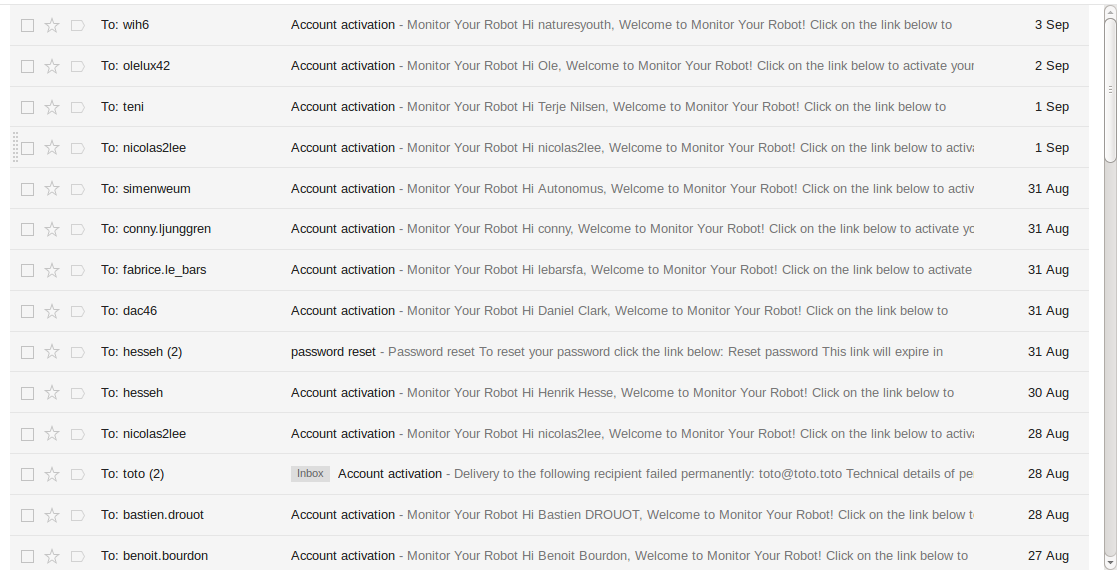
\includegraphics[width=15cm]{emailrecords.png}
\caption{Admin Gmail sending records}
\label{fig-sample}
\end{figure}

\begin{figure}[h!]
\centering
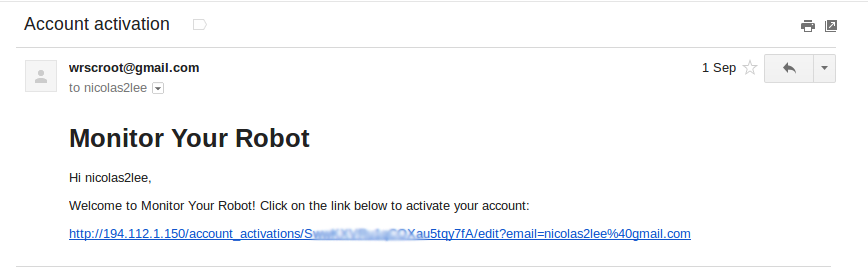
\includegraphics[width=12cm]{contentemail.png}
\caption{An example of activating email content}
\label{fig-sample}
\end{figure}

\item{\textbf{Tracking system}}


Here are some captures of missions:
\begin{figure}[h!]
\centering
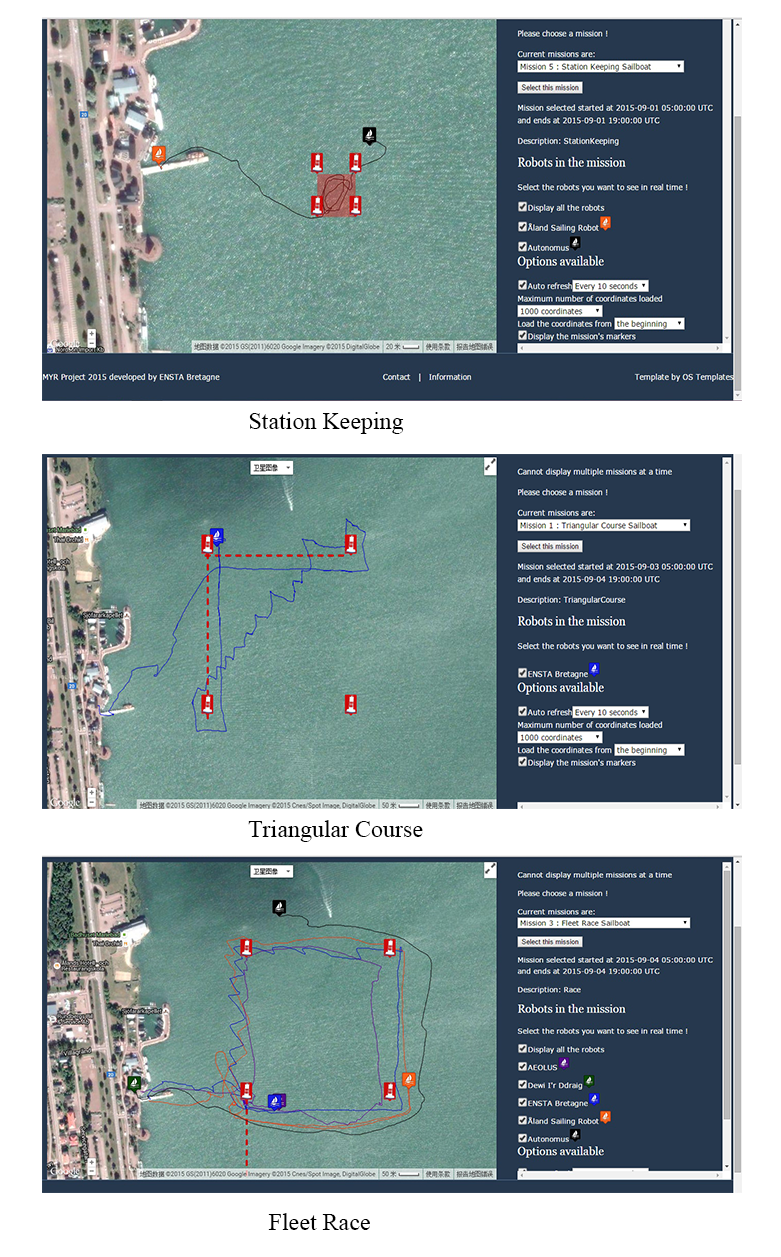
\includegraphics[width=12cm]{resultmissions.png}
\caption{Captures of WRSC mission in the real-time page }
\label{fig-sample}
\end{figure}
As the figures demonstrated, our web site could indicate the whole trace of all robots clearly, the tracking system works perfectly.

\item{\textbf{Scoring and Ranking}}

Before this year, all the scores were given by the Race committee and were measured by humans, but this year, with our tracking system and our algorithms, we can obtain more objective scores, so after discussing with the Race committee, the final result based on our calculations. Here is a quick view of the final standing:
\begin{figure}[h!]
\centering
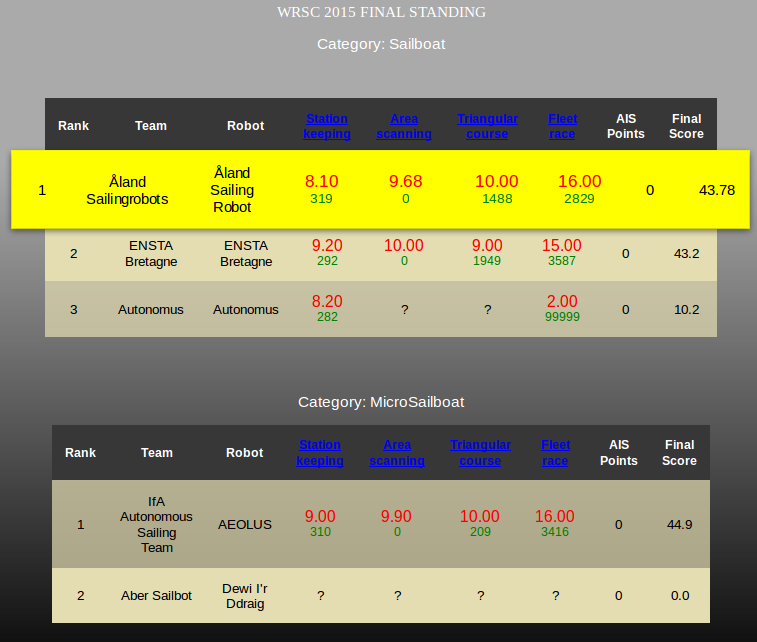
\includegraphics[width=12cm]{finalranking.png}
\caption{Final Standing of WRSC2015 }
\label{fig-sample}
\end{figure}
Also the uploading file function works well, and based on the submitted data and our trackers' data, here is a hint about the comparison of these two sets of data, finally the maximum difference is about 8 meters which is acceptable.
\begin{figure}[h!]
\centering
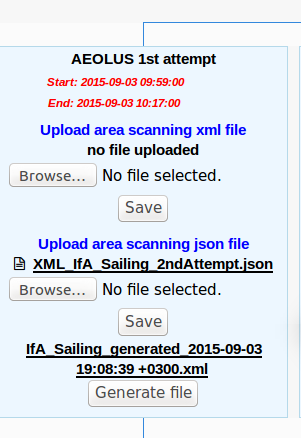
\includegraphics[width=8cm]{uploadingfiles.png}
\caption{Uploading file example }
\label{fig-sample}
\end{figure}
\begin{figure}[h!]
\centering
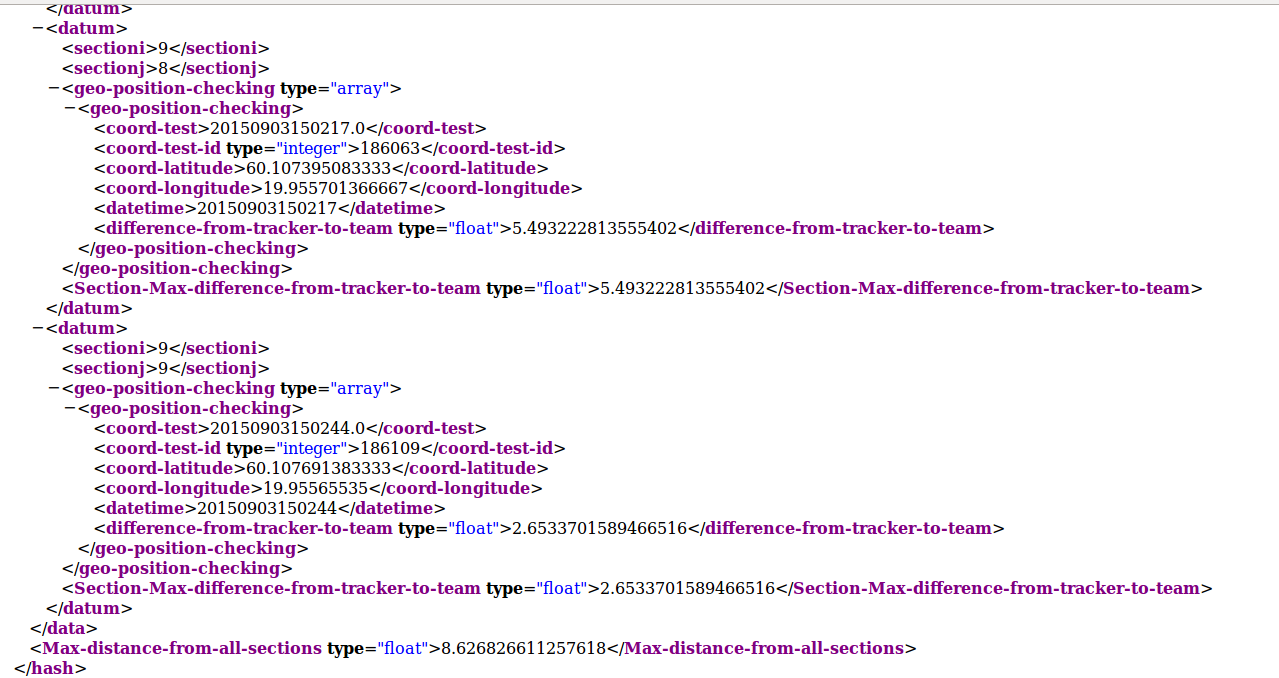
\includegraphics[width=12cm]{xmlfile.png}
\caption{old sign in }
\label{fig-sample}
\end{figure}
\end{enumerate}